\documentclass[authoryear,preprint,review,12pt]{elsarticle}

\usepackage{amssymb}
\usepackage{amsmath}
\usepackage{booktabs}
\usepackage{lineno}
\usepackage{hyperref}
\usepackage{graphicx}
\usepackage{tikz}
\usetikzlibrary{arrows.meta, positioning, fit, backgrounds}

\journal{Computers \& Geosciences}

\begin{document}

\begin{frontmatter}

\title{nowcast: a forcing-agnostic Rust engine for dynamic geohazard
nowcasting, and why forcing resolution, not the model, sets the skill ceiling}

\author[1]{Francisco Parra-O.\corref{cor1}}
\ead{francisco.parra.o@usach.cl}
\cortext[cor1]{Corresponding author}

\affiliation[1]{organization={Departamento de Ingenier\'ia Inform\'atica,
            Universidad de Santiago de Chile},
            city={Santiago},
            country={Chile}}

\begin{abstract}
Landslide and flood susceptibility maps are static: fixed predisposing factors
combined by physical or machine-learning models. Turning susceptibility into an
operational \emph{nowcast} requires modulating it in time with the dynamic
forcing that triggers failure, such as rainfall, snowmelt, routed discharge or
ground deformation. We present \textbf{nowcast}, a dependency-light Rust engine
that writes time-varying hazard as a susceptibility field times a trigger factor,
behind a single interchangeable forcing interface. The hazard logic is thereby
decoupled from the data source and from the trigger family. The engine ships
native providers that wrap sibling Rust models for rainfall--runoff, snowmelt,
2-D shallow-water inundation, an agent-based debris-flow model, a geospatial
raster substrate and PS-InSAR/SBAS deformation. Triggers are composable (rainfall
intensity--duration, discharge, deformation rate), and physical refinement runs
on demand only where the cheap nowcast alerts. We use the engine as an
experimental instrument over Chilean basins, holding the model fixed and varying
the resolution of the forcing. A backtest of 157 dated rainfall-triggered
landslides in the R\'io Maipo basin shows that the global Caine (1980)
intensity--duration threshold never fires on daily CR2MET forcing (probability of
detection, POD $=0$), whereas a calibrated regional intercept transfers
split-sample (validation POD $\approx 0.50$). Distributing that daily forcing
over the basin and weighting by a real machine-learning susceptibility raster
does not improve discrimination. The area under the ROC curve is indistinguishable
from random (AUC $\approx 0.48$; month-block bootstrap 95\,\% CI spans 0.5): at
5\,km daily resolution the gridded rainfall at event cell-months is no higher
than average, and a supervised baseline trained on the same daily features fares
no better (cross-validated AUC $\le 0.56$). A controlled experiment with known
ground truth illustrates the mechanism: the same engine discriminates planted
sub-daily bursts almost perfectly (AUC $\approx 1$), but aggregating the identical
field to daily resolution collapses the operational catch rate to effectively zero
(over 20 random realisations), with the model and terrain held fixed. The bottleneck is therefore the resolution of the
forcing rather than the model. At half-hourly GPM IMERG
resolution the same intensity--duration trigger pins the threshold crossing to a
timestamp hours ahead of the documented flows, whereas the same rain aggregated
to daily cannot trigger at all, because the finest resolvable mean intensity is
total$/24$\,h, smeared below the curve. We reproduce this contrast across three
dated events spanning opposite Chilean climates. A complementary flood path,
validated against observed daily streamflow on the R\'io Itata, discriminates
observed floods out of sample (ROC-AUC 0.90), because discharge routing integrates
the rainfall that a sub-daily landslide trigger must instead resolve directly. The
engine, its backtesting framework and all examples are open and reproducible.
\end{abstract}

\begin{highlights}
\item A forcing-agnostic Rust engine couples static susceptibility to dynamic triggers
\item Rainfall, snowmelt, discharge and InSAR deformation enter through one interface
\item Distributing daily rainfall does not improve discrimination (AUC $\approx 0.48$)
\item Forcing resolution, not the model, sets the intensity--duration skill ceiling
\item Half-hourly satellite forcing pins the threshold crossing hours ahead of flows
\end{highlights}

\begin{keyword}
nowcasting \sep landslides \sep floods \sep intensity--duration threshold \sep
rainfall resolution \sep Rust \sep early warning \sep Chile
\end{keyword}

\end{frontmatter}

\linenumbers

\section{Introduction}

Operational forecasting of rainfall-triggered geohazards sits between two
well-developed but disjoint bodies of work. On one side, \emph{susceptibility}
mapping combines static predisposing factors (slope, lithology, land cover,
terrain indices) through statistical, physically-based or, increasingly,
machine-learning models, to estimate \emph{where} failures are possible
\citep{reichenbach2018,merghadi2020}. On the other, empirical \emph{rainfall thresholds}, most
famously the intensity--duration (I--D) power law of \citet{caine1980} and its
many regional successors \citep{guzzetti2007,segoni2018,gariano2016}, estimate \emph{when}
triggering rainfall has occurred. Operational early-warning, however, needs
\emph{where} and \emph{when} together, as a hazard field that evolves through an
event \citep{bogaard2018}. This coupling is already realised operationally: NASA's
LHASA gates a static landslide susceptibility map with GPM IMERG satellite-rainfall
thresholds at the global scale \citep{kirschbaum2018}, its successor adds a
data-driven model \citep{stanley2021}, and geographical landslide early-warning
systems are now widespread \citep{guzzetti2020}. What these share is a
\emph{product-specific} design: the forcing, the trigger and the susceptibility
model are welded into one operational chain, so swapping the rainfall product,
adding a second trigger (snowmelt, discharge, deformation), or attaching a
physical-refinement model means rebuilding the pipeline. The open question is less
\emph{whether} to couple susceptibility and forcing than \emph{how much resolution
the forcing must carry} for the coupling to have skill, a question a fixed
operational chain cannot easily ask.

Closing that gap raises three software problems that recur across hazards and
regions. First, the \emph{forcing} is heterogeneous: a rain gauge, a gridded
reanalysis product, a satellite quantitative precipitation estimate, a
rainfall--runoff hydrograph, or an InSAR deformation field, each with its own
grid, units and time step. Second, the \emph{trigger} family is hazard-dependent:
landslides respond to rainfall I--D, floods to discharge over a threshold, slow
slopes to deformation rate, yet all share the structure ``exceedance of a
critical level mapped to a hazard factor''. Third, validation against dated event
inventories is itself a methods problem with non-obvious metric choices for rare,
spatially sparse, incomplete records.

We present \textbf{nowcast}, a Rust engine that addresses these three problems
with one abstraction (an interchangeable \emph{forcing} interface and a
composable \emph{trigger}), and we then use it as an experimental instrument to
ask a question rarely posed directly: holding the model fixed, how much does the
\emph{resolution of the forcing} determine attainable skill? The contributions
are computational rather than a new hazard law. (1)~A \emph{forcing-agnostic}
design whose random-access forcing trait makes online streaming and dated-event
replay backtesting fall out of one interface, so the same engine is both an
operational nowcaster and an experimental instrument, and the hazard logic never
changes when the rainfall product, the trigger family or the physical-refinement
model is swapped. (2)~A composable multi-trigger with \emph{exact, closed-form}
attribution of every alert, an analytic decomposition into terrain and forcing
drivers that needs no perturbation sampling (contrast SHAP), afforded by the
closed-form hazard. (3)~An on-demand coupling that confines expensive 2-D physics
to the cells the cheap nowcast has already flagged. (4)~A backtesting framework
with metrics appropriate for sparse, month-dated inventories, and the resolution
diagnosis that this instrument makes possible. The established components (the
Caine I--D law, a logistic factor, prefix-sum windows) enter as building blocks
and are not claimed as novel; the contribution is the architecture that makes
them independently swappable and the diagnosis that architecture enables. On real Chilean data, distributing daily forcing and
adding real susceptibility does not improve discrimination; this honest null,
with a sub-daily head-to-head, locates the binding constraint on the forcing
resolution rather than the model; a flood path validated against observed
streamflow shows the converse, where routing integrates the forcing, daily
resolution suffices (out-of-sample ROC-AUC 0.90).

\section{The nowcast engine}

\subsection{Hazard formulation}

The engine represents hazard on a row-major raster grid. For every cell and time
step,
\begin{equation}
\mathrm{hazard}(\mathrm{cell},t)=\mathrm{susceptibility}(\mathrm{cell})\times
\mathrm{trigger\_factor}(\mathrm{exceedance},t),
\label{eq:hazard}
\end{equation}
where $\mathrm{susceptibility}\in[0,1]$ is a static background field (a terrain
index, a physically-based factor-of-safety proxy, or a machine-learning
susceptibility raster) and $\mathrm{trigger\_factor}\in[0,1]$ is a dimensionless
modulation derived from the dynamic forcing. Both factors lie in $[0,1]$, so the
product is a bounded hazard index. We deliberately call it an \emph{index}, not a
calibrated probability (Section~\ref{sec:limits}).

The trigger factor is a smooth function of an \emph{exceedance ratio} $E$, how
far the forcing has crossed a critical level. A hard threshold ($E\geq 1$ fires,
else nothing) discards how far past the curve the forcing reached; instead we use
a logistic,
\begin{equation}
\mathrm{trigger\_factor}(E)=\frac{1}{1+\exp\!\big(-k\,(E-1)\big)},
\label{eq:logistic}
\end{equation}
with $\mathrm{trigger\_factor}(1)=0.5$ exactly on the curve and steepness $k$
(default 4). The \emph{source} of $E$ is what varies between hazards.

\subsection{The forcing interface}

A single trait abstracts the dynamic forcing as a per-cell, per-step scalar field
with a known time step:
\begin{verbatim}
pub trait Forcing {
    fn dims(&self) -> GridDims;
    fn n_steps(&self) -> usize;
    fn dt_hours(&self) -> f64;
    fn depth_mm(&self, cell: usize, step: usize) -> f64;
}
\end{verbatim}
Random access (rather than a pull/iterator model) is deliberate: the I--D logic
accumulates rolling windows, and backtesting replays whole dated series. Shipped
implementations are a single observed gauge broadcast over a grid, an independent
series per cell (a gridded precipitation product) and, through the provider
crates, snowmelt runoff and InSAR deformation. The same trait therefore admits a
gauge, a reanalysis grid, a satellite product or a model output without touching
the hazard logic (Fig.~\ref{fig:arch}).

\begin{figure}[t]
\centering
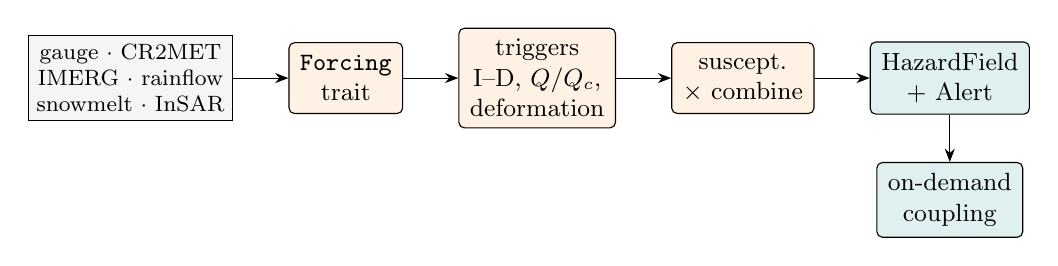
\begin{tikzpicture}[font=\small, >=Stealth,
  box/.style={draw, rounded corners=2pt, align=center, inner sep=4pt, minimum height=9mm},
  src/.style={draw, align=center, inner sep=3pt, font=\footnotesize, fill=black!4},
  core/.style={box, fill=orange!10},
  outbox/.style={box, fill=teal!12}]
\node[src] (forc) {gauge $\cdot$ CR2MET\\ IMERG $\cdot$ rainflow\\ snowmelt $\cdot$ InSAR};
\node[core, right=7mm of forc] (trait) {\texttt{Forcing}\\ trait};
\node[core, right=7mm of trait] (trig) {triggers\\ I--D, $Q/Q_c$,\\ deformation};
\node[core, right=7mm of trig] (haz) {suscept.\\ $\times$ combine};
\node[outbox, right=7mm of haz] (alert) {HazardField\\ + Alert};
\node[outbox, below=6mm of alert] (couple) {on-demand\\ coupling};
\draw[->] (forc)--(trait); \draw[->] (trait)--(trig); \draw[->] (trig)--(haz);
\draw[->] (haz)--(alert); \draw[->] (alert)--(couple);
\end{tikzpicture}
\caption{Engine dataflow. Heterogeneous forcings enter through one
\texttt{Forcing} interface; composable triggers map each to an exceedance factor;
their combination modulates the static susceptibility into a per-step
\texttt{HazardField} and \texttt{Alert}s. Where an alert fires, a process model is
run on demand to refine it (2-D shallow water for floods, an agent-based
debris-flow model for landslides). The geospatial substrate (GeoTIFF I/O, CRS)
moves rasters in and out.}
\label{fig:arch}
\end{figure}

\subsection{The rainfall intensity--duration trigger}

For rainfall-triggered landslides the exceedance is computed against a power-law
I--D curve,
\begin{equation}
I_{\mathrm{crit}}(D)=a\,D^{-b}\qquad(I\;\mathrm{in\;mm\,h^{-1}},\;D\;\mathrm{in\;h}),
\label{eq:id}
\end{equation}
with the \citet{caine1980} global intercept $a=14.82$, $b=0.39$ as a default,
replaceable by a regional curve. For each cell and step, the engine accumulates
water input over rolling windows of length $m=1\ldots m_{\max}$ ending at that
step, forms the mean intensity $I=\mathrm{depth}/(m\,dt)$ and duration $D=m\,dt$,
evaluates $E_m=I/I_{\mathrm{crit}}(D)$, and takes the worst (maximum) exceedance
over all windows; per-cell prefix sums make each window sum $O(1)$.

\subsection{Composable triggers}

The engine generalises the trigger to \emph{composable exceedance sources}. A
\texttt{Trigger} yields a factor per cell and step; an \texttt{IdTrigger}
implements the rolling-window I--D logic above; a \texttt{ThresholdTrigger}
implements a duration-independent exceedance $E=\mathrm{value}/\mathrm{value_{crit}}$
suitable for any signal already expressed as a rate (routed discharge $Q/Q_c$,
InSAR velocity $|v|/v_{\mathrm{crit}}$). A \texttt{MultiNowcast} fuses several
triggers through a combination rule before modulating susceptibility:
\begin{equation}
\mathrm{hazard}=\mathrm{susceptibility}\times\mathrm{combine}(f_1,\ldots,f_k),
\quad\mathrm{combine}\in\{\max,\ \mathrm{noisy\text{-}OR},\ \mathrm{product}\}.
\label{eq:multi}
\end{equation}
Noisy-OR ($1-\prod(1-f_i)$) is the natural rule for independent triggers where
any one may fire, for example \emph{rain I--D} OR \emph{deformation rate}. The
per-trigger factors are exposed for traceability.

\subsection{Physical refinement on demand}

The susceptibility$\times$trigger product is a fast, coarse screen. Where it
alerts, the engine couples, one-way and on demand, to a process model that
refines the alert into a physical field, only over the alerted area. For
\textbf{floods}, a 2-D shallow-water solver (HLLC fluxes, Audusse well-balanced
reconstruction \citep{audusse2004}, semi-implicit Manning friction) routes the
alerting discharge over the local digital elevation model and returns an
inundation depth per cell. For \textbf{landslides/debris flows}, an agent-based
model (rain and flow agents over the terrain raster, calibrated on the 2015
Atacama event) returns the runout footprint. That calibration feeds only the
runout-footprint demonstration and is independent of the I--D lead-time analysis
(Section~5.4), which uses the rainfall trigger alone. In both, the coarse probability is
downscaled onto the physical footprint; the expensive model runs only where the
cheap nowcast already alerted. The saving is the point and is quantifiable:
because the shallow-water solver integrates to a fixed physical time with
CFL-limited steps, its cost is ${\sim}O(\mathrm{cells})$, so confining it to an
alerted tile spanning 31\,\% of a coarse domain runs $3.9\times$ faster than
solving the full domain (1.19\,s to 0.31\,s) while returning \emph{bit-identical}
depths in the inundated region, the flood being contained within the tile. The
on-demand restriction is therefore free in accuracy, and the cheap
susceptibility$\times$trigger screen is what keeps the alerted area, and hence the
hydrodynamic cost, small.

\subsection{Exact attribution}

Because Eq.~\eqref{eq:hazard} is closed-form, every alert is \emph{exactly}
attributable, there is no surrogate model to approximate, as post-hoc methods
such as SHAP \citep{lundberg2017} require for black boxes. For any cell and step
the engine reports the two factors, the rolling I--D window that drove the trigger
(its duration, mean intensity, critical intensity and exceedance), which
side, terrain or forcing, is the binding constraint, and a counterfactual: the
rainfall intensity, at a given duration, that would lift the cell to the alert
level. SHAP remains relevant one layer upstream, explaining the machine-learning
\emph{susceptibility} that enters Eq.~\eqref{eq:hazard} as an
already-interpretable input.

\subsection{Implementation}

The engine is written in Rust (edition 2024) as a Cargo workspace of ten
crates. The core depends only on \texttt{std} and an error-handling crate, so it
builds and tests offline with no system dependencies; native providers are
separate crates that wrap sibling engines through path dependencies:
rainfall--runoff (GR4J/HBV; \citealp{perrin2003,seibert2012}), distributed
snowmelt, 2-D shallow water \citep{audusse2004,toro1994}, an agent-based
debris-flow model in the cellular-automata tradition \citep{dambrosio2003}, the geospatial raster substrate (native GeoTIFF I/O, no GDAL
dependency), PS-InSAR/SBAS deformation \citep{ferretti2001,berardino2002}, and a wildfire-spread model (Rothermel surface-fire spread \citep{andrews2018} with a minimum-travel-time perimeter algorithm \citep{finney1998}) with a
post-fire susceptibility cascade; a command-line runner exposes the engine
(run, backtest, explain, watch, calibrate) and PyO3 bindings expose it to Python. The codebase is covered by
$\sim$58 unit and documentation tests, the linter runs clean under
\texttt{-D warnings}, and twenty-eight runnable examples reproduce every result below.
Each provider is a dependency-isolated crate implementing the same \texttt{Forcing}
trait, so the design is reusable and extensible by construction: adding a hazard
forcing is a new crate, not an edit to the core. That separation, not any single
algorithm it orchestrates, is the engine's computational contribution.

\subsection{Computational performance}

The I--D engine is $O(\mathrm{cells}\times\mathrm{steps}\times m_{\max})$: per-cell
prefix sums reduce each rolling-window sum to $O(1)$, and memory is
$O(\mathrm{cells}\times\mathrm{steps})$ for the prefix buffer. On a single core
(release build, $m_{\max}=7$), throughput is roughly constant at
${\sim}3.7$~million cell-steps per second, confirming the linear scaling
(Table~\ref{tab:perf}). In practice the lumped Maipo backtest (270 cells $\times$
13\,880 daily steps $\approx 3.7$~M cell-steps) runs in about one second, and a
seasonal continental-scale run (490\,k cells $\times$ 365 steps $\approx$
179~M cell-steps) in under a minute. An optional Rayon backend
(\texttt{--features parallel}) parallelises the independent per-step loop; the
closure captures only the read-only prefix buffer, so the output is bit-identical
to the serial run. The speed-up is, however, modest and bandwidth-bound: on a
16-core machine over a 50~M cell-step grid it reaches $1.8\times$ on 2 threads
(88\,\% efficiency) but saturates at $2.8\times$ on 16 threads
(Table~\ref{tab:scaling}), because each step does little arithmetic per byte read
and the shared prefix buffer makes the loop memory-bandwidth-bound rather than
compute-bound. The $O(\mathrm{cells}\times\mathrm{steps})$ prefix buffer
(${\sim}1.4$~GB at the largest size above) is the practical memory limit,
mitigated by chunking the time axis; that same memory pressure, not a lack of
parallel work, is what caps the multi-thread speed-up.

\begin{table}[ht]
\centering
\caption{Single-thread runtime of \texttt{Nowcast::run} over synthetic grids.}
\label{tab:perf}
\begin{tabular}{@{}rrrrr@{}}
\toprule
cells & steps & cell-steps & time (s) & M\,cell-steps\,s$^{-1}$ \\
\midrule
10\,000  & 60  & 0.6\,M   & 0.17  & 3.6 \\
90\,000  & 200 & 18\,M    & 4.7   & 3.8 \\
250\,000 & 200 & 50\,M    & 11.2  & 4.5 \\
490\,000 & 365 & 179\,M   & 48.1  & 3.7 \\
\bottomrule
\end{tabular}
\end{table}

\begin{table}[ht]
\centering
\caption{Parallel scaling of \texttt{Nowcast::run} (\texttt{--features parallel})
over a 50~M cell-step grid, 16-core machine, best of two runs. Output is verified
bit-identical to the single-thread run.}
\label{tab:scaling}
\begin{tabular}{@{}rrrr@{}}
\toprule
threads & time (s) & speed-up & efficiency \\
\midrule
1  & 10.5 & 1.0$\times$ & 100\,\% \\
2  & 6.0  & 1.8$\times$ & 88\,\% \\
4  & 5.2  & 2.0$\times$ & 50\,\% \\
8  & 4.2  & 2.5$\times$ & 31\,\% \\
16 & 3.7  & 2.8$\times$ & 18\,\% \\
\bottomrule
\end{tabular}
\end{table}

\section{Data and study area}

All experiments use openly documented Chilean datasets (Table~\ref{tab:data}).
Susceptibility is a RandomForest probability raster at 30\,m resolution (values
0.001--0.965 over the R\'io Maipo basin, $5149\times5855$ cells), taken from a
companion susceptibility study: the model is trained on landslide presence points
from the SERNAGEOMIN catalogue (augmented with the Patagonian-Andes and 2010 Maule
co-seismic inventories) against spatially-interspersed absence points and terrain,
geology and climate predictors, under spatial cross-validation. This raster is
therefore \emph{not independent} of the validation inventory: it was trained on a
superset of the same dated events the backtest scores against. The dependence is,
however, \emph{conservative} for our purpose. Leakage can only \emph{inflate} the
susceptibility's apparent agreement with event locations, so an inventory-informed
susceptibility that still fails to discriminate at 5\,km daily resolution
(Section~5.2) strengthens the resolution-ceiling conclusion rather than weakening
it; we flag the single place the dependence could matter (the weak single-feature
susceptibility signal in the baseline) where it arises. Daily
precipitation is CR2MET v2.5 (0.05$^\circ$, $\sim$5\,km; \citealp{boisier2018cr2met}), produced over a basin
region that has experienced a sustained decline in rainfall since 2010, the
Central Chile Mega Drought \citep{garreaud2019,boisier2018}.
Sub-daily precipitation is GPM IMERG Final v07 half-hourly ($\sim$0.1$^\circ$;
\citealp{huffman2020,tan2019}). Catchment forcing for the flood path uses CAMELS-CL
\citep{alvarez2018}. The dated event inventory is the SERNAGEOMIN
landslide/flow catalogue, consistent with regional patterns of rainfall-triggered
fatal landslides across Chile and Latin America \citep{sepulveda2015}; events are dated to year and month from the record
identifier, and the month itself is only approximate: the Atacama event flows,
for instance, are filed under March even though the extreme rainfall fell over
24--26 March 2015.

\begin{table}[ht]
\centering
\caption{Datasets.}
\label{tab:data}
\begin{tabular}{@{}llll@{}}
\toprule
Dataset & Variable & Resolution & Use \\
\midrule
RandomForest susceptibility & susceptibility & 30\,m & static background \\
CR2MET v2.5 & daily precipitation & 0.05$^\circ$, daily & lumped \& distributed forcing \\
GPM IMERG Final v07 & precipitation rate & $\sim$0.1$^\circ$, 30\,min & sub-daily forcing \\
CAMELS-CL & precip, PET, streamflow & catchment, daily & flood path (GR4J/HBV) \\
SERNAGEOMIN inventory & dated events & point, $\sim$month & validation target \\
\bottomrule
\end{tabular}
\end{table}

Study sites are the R\'io Maipo basin (central Andes, landslide backtest), the
R\'io Itata catchment (humid south-central, flood path), and three dated
debris-flow events spanning opposite climates: Atacama/Copiap\'o (25 March 2015,
arid, convective), Caj\'on del Maipo (25 February 2017, central Andes, summer
convective) and Villa Santa Luc\'ia (16 December 2017, humid south, frontal). They
span roughly $27^\circ$S to $43^\circ$S, from the hyper-arid Atacama to the humid
Patagonian Andes (Fig.~\ref{fig:studyarea}).

\begin{figure}[t]
\centering
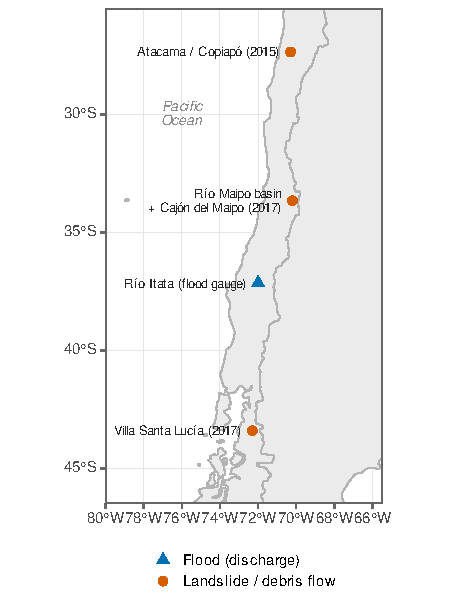
\includegraphics[width=0.48\linewidth]{figs/fig1_studyarea.pdf}
\caption{Study sites in Chile, spanning the arid north to the humid south. Orange:
landslide/debris-flow sites, the R\'io Maipo landslide backtest, which also hosts the
25 February 2017 Caj\'on del Maipo event, the 25 March 2015 Atacama/Copiap\'o event
and the 16 December 2017 Villa Santa Luc\'ia event. Blue: the R\'io Itata
flood-validation catchment (CAMELS-CL gauge 8123001).}
\label{fig:studyarea}
\end{figure}

\section{Methods}

\subsection{Backtesting metrics}

Validation of a nowcast is binary forecast verification, giving a $2\times2$
contingency table and the standard categorical scores, probability of detection
(POD), false-alarm ratio (FAR), critical success index (CSI), frequency bias.
Because the inventory is dated only to $\sim$month, the matching unit is the
calendar month, and matching is \emph{event-centred} with a $\pm$tolerance window
(an event is a hit if an alert falls within the window; a false alarm is an
alerted month far from any event) to avoid inflating misses when one event spans
a tolerance window. For \emph{spatial} verification, per-cell month matching
against a spatially sparse, \emph{incomplete} inventory makes CSI/FAR
meaningless, almost every ``false alarm'' is a susceptible, wet cell with no
\emph{recorded} event. We therefore score discrimination, as the susceptibility
and early-warning literatures do \citep{reichenbach2018}: ROC-AUC \citep{hanley1982} (does the hazard
rank event cell-months above quiet ones?) and POD at a fixed alerted-area
fraction. Uncertainty on the AUC is estimated by a \emph{month-block} bootstrap
(resampling calendar months with replacement, keeping each month's cells
together) so that within-month spatial autocorrelation, the dominant structure
when one storm wets many cells, is not mistaken for independent information. As a
model-agnostic check, we also train supervised baselines (logistic regression and
gradient boosting \citep{friedman2001}) on per-cell-month susceptibility and rainfall features,
evaluated by year-blocked \texttt{GroupKFold} cross-validation, chosen over a
plain random split to avoid leaking within-year spatial autocorrelation across
folds \citep{roberts2016}.

We distinguish two notions used throughout the results. \emph{Triggering} asks
whether the forcing can cross the I--D curve at all; it is a property of the
intensity at the finest resolvable duration, and a daily product can fail it
structurally (Section~5.4). \emph{Discrimination} (or skill) asks the harder
question of whether the resulting hazard \emph{ranks} event locations above
non-event ones, as ROC-AUC and POD measure. The two are not interchangeable: a
forcing can trigger frequently yet discriminate poorly. The distributed backtest
(Section~5.2) tests discrimination on real but month-dated data; a controlled
synthetic experiment (Section~5.3) tests it under known ground truth; the
head-to-head (Section~5.4) isolates triggering.

\subsection{Threshold calibration and split-sample validation}

The I--D intercept $a$ is calibrated by sweeping it (fixed $b=0.39$) and selecting
the value that maximises CSI against the dated events; $k=4$ and a maximum rolling
window of 7\,days (storm I--D durations, not seasonal accumulation) are fixed.
The steepness $k$ enters only through the trigger factor (Eq.~\ref{eq:logistic}),
which is monotonic in the exceedance, so the rank-based discrimination scores
(ROC-AUC, POD at a fixed area) are \emph{exactly} invariant to $k$ for the
trigger-only configuration, where the hazard is a monotone function of exceedance;
$k$ enters the threshold-based POD/FAR only through the chosen alert level.
Validation is split-sample: the intercept is calibrated on odd calendar years and
evaluated on even years.

\section{Results}

\subsection{Lumped landslide backtest (R\'io Maipo)}

Over 13\,880 daily steps (1979--2016) and 157 dated rainfall-triggered events, the
global Caine threshold ($a=14.82$) \textbf{never fires} on CR2MET daily forcing
(POD $=0$): the daily-mean intensity of even the wettest days sits below the curve
at 24\,h duration. A calibrated regional intercept $a^\star\approx5.5$\,mm\,h$^{-1}$
is robust, the full-period and odd-year calibrations agree, and transfers
split-sample (validation POD $\approx 0.50$; Fig.~\ref{fig:idsweep}). The
false-alarm ratio is high (FAR $\approx 0.92$) but structural: with an event base rate near 4\,\% and a
single representative gauge in a Mediterranean wet-season climate, an I--D trigger
alone over-predicts. The inventory's month-level dating caps attainable POD:
widening the match tolerance from $\pm0$ to $\pm3$ months raises POD from 0.21 to
0.68 (Table~\ref{tab:lumped}), so a large share of ``misses'' is date error in the
inventory, not model error.

\begin{table}[ht]
\centering
\caption{Lumped Maipo backtest (monthly contingency, $\pm1$-month match unless noted).}
\label{tab:lumped}
\begin{tabular}{@{}lccl@{}}
\toprule
Configuration & POD & FAR & note \\
\midrule
Caine global, $a=14.82$ & 0.00 & 1.00 & never fires \\
Regional $a^\star=5.5$ (full period) & 0.53 & 0.92 & max-CSI calibration \\
Regional $a^\star=5.5$ (split-sample) & 0.50 & 0.93 & calibrate odd $\to$ validate even \\
$a^\star=5.5$, tol. $\pm0/\pm1/\pm2/\pm3$\,mo & \multicolumn{2}{c}{POD 0.21/0.53/0.58/0.68} & inventory date noise \\
\bottomrule
\end{tabular}
\end{table}

\begin{figure}[t]
\centering
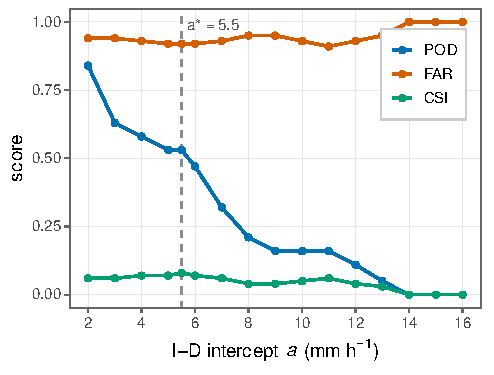
\includegraphics[width=0.62\linewidth]{figs/fig2_idsweep.pdf}
\caption{Calibration of the I--D intercept $a$ on the lumped Maipo backtest
(monthly contingency, $\pm1$-month match). POD falls and false-alarm ratio stays
high across the sweep; the critical success index peaks at $a^\star\approx5.5$\,mm\,h$^{-1}$
(dashed line), far below the Caine global value of 14.82.}
\label{fig:idsweep}
\end{figure}

\paragraph{Published thresholds do not rescue daily forcing.}
Self-calibration invites the objection that a published threshold, taken as is,
might do better. We tested this directly by applying, unchanged, the 35 empirical
I--D power laws ($I=a\,D^{-b}$, mm\,h$^{-1}$) compiled by \citet{guzzetti2007}
(their Table~2, the canonical collation of the literature) to the same CR2MET
daily forcing. The outcome is dictated by resolution, not by the curve: 10 of the
35 sit \emph{structurally} above the daily ceiling --- on a basin whose wettest
day in 38 years is 136\,mm, no daily forcing can reach their 24\,h intensity, since
the maximum resolvable 24\,h intensity is the daily total divided by 24 --- and 5
never fire at all. Thirteen yield POD $=0$, and of the curves that do fire, 30 have
FAR $\geq 0.90$. The best-scoring published curve attains CSI $=0.084$,
indistinguishable from the self-calibrated regional intercept (CSI $=0.077$): the
entire ensemble is pinned near the same low operating point. A curve high enough to
be selective sits above the wettest day (POD $0$); lowered enough to fire, it fires
on most wet months (FAR $\to 1$). The binding constraint is the forcing resolution,
not the choice of published threshold (\texttt{published\_thresholds} example).

\subsection{Distributed daily backtest, an honest null}

Repeating the backtest with \emph{distributed} CR2MET rainfall over a
$15\times18$ grid (270 cells, 123\,120 cell-months, 884 in the event footprint),
the \emph{real} RandomForest susceptibility resampled to that grid, and spatial
verification, yields essentially \textbf{no discrimination}
(Table~\ref{tab:auc}): ROC-AUC is 0.463 for a lumped basin-mean baseline
weighted by susceptibility, 0.477 for distributed rainfall with uniform
susceptibility, and 0.485 for distributed rainfall weighted by real
susceptibility. A month-block bootstrap (resampling months with replacement, so
within-month spatial autocorrelation is preserved; $B=2000$) puts all three 95\,\%
confidence intervals across the random 0.5 ($[0.40, 0.57]$ for the best
configuration), and the bootstrap probability that AUC exceeds 0.5 is only
0.21--0.34. None of the configurations is distinguishable from random. The mean
7-day rainfall at recorded event cell-months (45\,mm) is in fact \emph{lower}
than the grid-wide average (49\,mm).
At 5\,km daily resolution the gridded rainfall does not discriminate where and
when these landslides were recorded, and 30\,m susceptibility averaged to 5\,km
loses its edge. Distributing the forcing does not help: the limiting factor is the
\emph{resolution} of the forcing and susceptibility (and the month-level
inventory), not the lumping.

\begin{table}[ht]
\centering
\caption{Distributed-backtest discrimination (ROC-AUC) with month-block
bootstrap 95\,\% confidence intervals ($B=2000$). Every interval spans 0.5.}
\label{tab:auc}
\begin{tabular}{@{}lccc@{}}
\toprule
configuration & AUC & 95\,\% CI & $P(\mathrm{AUC}>0.5)$ \\
\midrule
lumped (basin-mean) $\times$ susc. & 0.463 & $[0.375, 0.550]$ & 0.21 \\
distributed, susc.\ $=1$           & 0.477 & $[0.399, 0.560]$ & 0.30 \\
distributed $\times$ real susc.    & 0.485 & $[0.403, 0.565]$ & 0.34 \\
\bottomrule
\end{tabular}
\end{table}

A supervised baseline confirms this is a property of the data, not of our
trigger. Logistic regression and gradient boosting trained on per-cell-month
features (susceptibility; monthly total; maximum 1-day and 7-day rainfall;
previous-month total), evaluated with year-blocked \texttt{GroupKFold}, reach a
cross-validated AUC of only 0.56 and 0.52, barely above random. A single-feature
analysis locates the little signal that exists: it comes from the static
susceptibility (AUC 0.55, itself an optimistic upper bound since this raster was
trained on the same inventory, Section~3) and weak antecedent wetness (0.52),
whereas every rainfall-intensity feature is at or below random (max 7-day 0.49,
max 1-day 0.46, monthly total 0.46). The daily rainfall therefore carries essentially no
information about where and when these landslides occurred, and a flexible model
cannot recover a signal the daily product does not contain. Our engine's 0.485
even dips slightly below susceptibility alone, because multiplying susceptibility
by a near-random daily-rainfall factor dilutes it: at this resolution the daily
trigger is worse than none.

\begin{figure}[t]
\centering
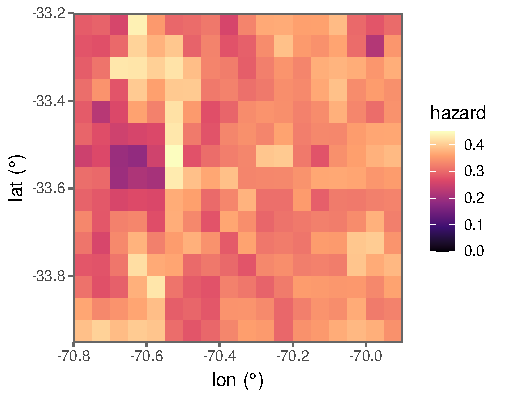
\includegraphics[width=0.6\linewidth]{figs/fig4_hazard.pdf}
\caption{Example distributed hazard field over the R\'io Maipo event region
(15$\times$18 CR2MET grid) at the wettest step, with real RandomForest
susceptibility and the regional I--D trigger ($a=5.5$). The field is
spatially structured, yet at 5\,km daily resolution it does not separate the
recorded event cell-months (Section~5.2); Fig.~\ref{fig:synthetic} shows, on
controlled data, how that discrimination returns as resolution increases.}
\label{fig:hazard}
\end{figure}

\subsection{Controlled resolution experiment}
\label{sec:synthetic}

The distributed null is ambiguous on its own: a near-random AUC could mean the
engine has no skill, or that the month-dated, incomplete inventory cannot reveal
skill that is present. We resolve the ambiguity with a controlled experiment whose
ground truth is known by construction. On a $20\times20$ grid over 60 days we
synthesise one half-hourly rainfall field in which the \emph{only} feature that
separates an event cell-day from a non-event cell-day is the sub-daily intensity
profile, not the daily total: event cell-days deliver a modest total (16--26\,mm)
as a ${\sim}1$\,h convective burst that crosses the I--D curve, while
\emph{confounder} cell-days deliver a similar or larger total (16--46\,mm) smeared
over 16--23\,h, so their intensity stays below the curve. The same active cells
host both kinds of day, so the static susceptibility carries no information that
distinguishes them and discrimination must come from resolving the burst. We then
aggregate the identical field to coarser resolution (0.5\,h to 24\,h), holding the
I--D engine and the 24\,h maximum duration fixed, and score discrimination of the
planted events at each resolution, averaged over 20 random realisations
(Fig.~\ref{fig:synthetic}).

At half-hourly resolution the engine recovers the planted events almost perfectly
(ROC-AUC $1.00\pm0.00$ on the trigger alone; $0.88\pm0.02$ once multiplied by the
structured susceptibility, which here adds noise but no signal) and the operational
catch rate is high (POD at a 5\,\% alerted-area budget $0.37\pm0.10$). As the field
is aggregated the maximum resolvable mean intensity falls toward total$/24$\,h, the
bursts smear below the curve, the trigger rate drops from 35\,\% to 18\,\% of
cell-days, the trigger-only AUC decays monotonically (to $0.79\pm0.01$; multiplied
by the structured susceptibility it ends at $0.81\pm0.02$ after a shallow,
noise-driven plateau), and the operational catch rate \textbf{collapses to
POD@5\,\% $=0.002\pm0.005$, i.e.\ effectively zero,} at daily resolution: with a
realistic alert budget a daily product catches essentially \emph{none} of the
events a sub-daily product catches. The residual daily AUC above 0.5 is, if
anything, the optimistic case for daily forcing, the synthetic events still carry an
above-dry daily total; in the real Maipo data even that vanishes, because recorded
event cell-months are no wetter than average (Section~5.2). The experiment isolates
the \emph{aggregation mechanism} under known ground truth, the engine discriminates
when the triggering signal is temporally resolved and loses that skill under
aggregation, with model and terrain fixed; it is a demonstration of the mechanism,
not a claim about real-event base rates, which the field backtests
(Sections~5.1--5.2) address.

\begin{figure}[t]
\centering
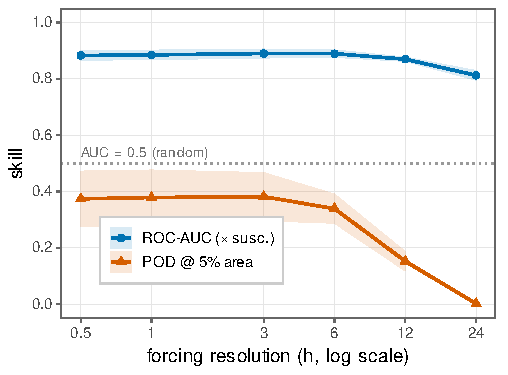
\includegraphics[width=0.6\linewidth]{figs/fig_synthetic.pdf}
\caption{Controlled resolution experiment (mean over 20 random realisations; bands
$\pm1$ sd). Synthetic half-hourly rainfall fields with planted convective-burst
events and same-total spread-rain confounders, aggregated to coarser resolution
(log axis) under a fixed I--D engine and 24\,h maximum duration. Discrimination of
the planted events, ROC-AUC weighted by susceptibility (blue) and POD at a 5\,\%
alerted-area budget (orange), is high at sub-hourly resolution and collapses toward
daily, the operational catch rate to effectively zero. The engine discriminates when the burst
is resolved; daily aggregation (intensity capped at total$/24$\,h) destroys the
skill, with the model and terrain held fixed.}
\label{fig:synthetic}
\end{figure}

\subsection{Resolution head-to-head}

The previous null motivates a controlled comparison of forcing resolution on the
same storm core (Atacama, 24--26 March 2015; the IMERG event-total maximum at
lon $-70.45$, lat $-27.15$), with the identical I--D engine
(Table~\ref{tab:headtohead}). The core is selected \emph{conditional on the known
event}, so this is a triggering-timing comparison, can each product cross the curve,
and when, not a discrimination test; discrimination is the business of the
distributed backtest (Section~5.2) and the controlled experiment
(Section~\ref{sec:synthetic}). With a daily value the finest resolvable duration is
24\,h, so the maximum resolvable mean intensity is (daily total)$/24$\,h: CR2MET
sees 30.1\,mm spread to 0.66\,mm\,h$^{-1}$, an exceedance of at most 0.62
(regional $a=4.0$) or 0.17 (Caine), the daily product \textbf{structurally cannot
trigger}, regardless of total. The same storm core in half-hourly IMERG peaks at
40\,mm\,h$^{-1}$; the I--D threshold is crossed at 04:30 UTC on 24 March
($E\approx12$), hours before the documented flows (Fig.~\ref{fig:leadtime}).
Higher-resolution forcing overcomes the limit with no change to the engine. The
two products also disagree on magnitude (IMERG 108\,mm vs CR2MET 30\,mm at this
core); IMERG is known to overestimate in arid convective regimes while CR2MET,
gauge-blended over a near-ungauged zone, likely underestimates, so the true
total lies between. Crucially, the resolution argument is \emph{independent} of
this: even taking CR2MET's own 30\,mm total, spreading it over 24\,h yields a
mean intensity far below the I--D curve, so a daily product cannot trigger
regardless of which magnitude is correct.

\begin{table}[ht]
\centering
\caption{CR2MET daily vs.\ GPM IMERG half-hourly at the Atacama storm core (same I--D engine).}
\label{tab:headtohead}
\begin{tabular}{@{}lcc@{}}
\toprule
 & CR2MET daily ($\sim$5\,km) & IMERG $\frac{1}{2}$-hourly ($\sim$10\,km) \\
\midrule
event total & 30.1\,mm & 108.5\,mm \\
finest resolvable duration & 24\,h & 0.5\,h \\
max resolvable intensity & 0.66\,mm\,h$^{-1}$ & 40.0\,mm\,h$^{-1}$ \\
I--D ($a=4.0$) & no alert ($E\leq0.62$) & alert 24-Mar 04:30 ($E\approx12$) \\
\bottomrule
\end{tabular}
\end{table}

\begin{figure}[t]
\centering
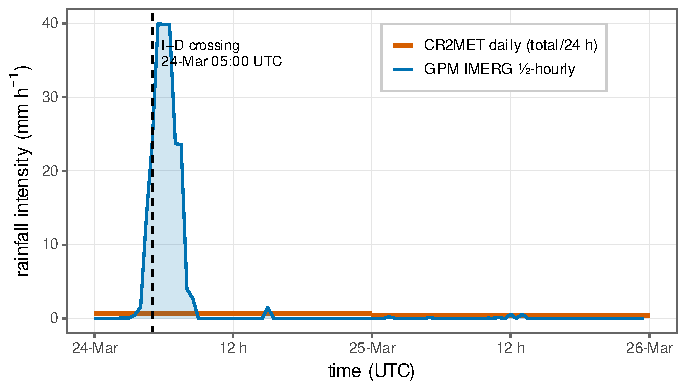
\includegraphics[width=0.78\linewidth]{figs/fig3_leadtime.pdf}
\caption{Forcing resolution at the Atacama storm core (24--26 March 2015). The
GPM IMERG half-hourly intensity (blue) peaks at 40\,mm\,h$^{-1}$ and crosses the
I--D curve at 04:30 UTC on 24 March; the same rainfall seen by a daily product
(CR2MET, orange: total$/24$\,h) is a flat ${\sim}1$\,mm\,h$^{-1}$ that never
reaches the curve. The daily product structurally cannot resolve the
triggering burst.}
\label{fig:leadtime}
\end{figure}

\subsection{Multi-event sub-daily lead time}

The sub-daily result generalises across three dated debris-flow events in opposite
climates (Table~\ref{tab:multievent}). In all three the half-hourly I--D crossing
lands on or just before the documented day. For the Caj\'on del Maipo summer
convective burst, the same rainfall aggregated to daily \textbf{never triggers}, only
sub-daily resolution detects it. The inventory provides no event onset \emph{hour},
so these are not formal lead-time skill scores but a demonstration that sub-daily
forcing resolves the threshold-crossing time that daily forcing cannot.

As a spatial false-alarm check, we ran the identical per-cell I--D trigger over each
event's full IMERG scene. The documented storm core is in every case the most
extreme cell (96.7--100th percentile of peak exceedance), but the trigger crosses
the curve over a broad footprint, 41\,\% of the Atacama scene, 16\,\% at Caj\'on del
Maipo, and the entire (small, frontal) Villa Santa Luc\'ia box, so the crossing is
not spatially sparse within these storm-centred scenes. This locates the \emph{peak}
correctly but is \emph{not} a low false-alarm rate, and because the box is
event-centred by construction a high crossing fraction is expected. A genuine
discrimination estimate needs the off-event crossing frequency at these cores, a
multi-year sub-daily record on days \emph{without} a documented flow, which the
present event-window granules do not provide. The sub-daily results are therefore
triggering-timing demonstrations, not skill scores; assembling that multi-year
sub-daily record is, with a day-resolution inventory (Section~7), the key remaining
validation step.

\begin{table}[ht]
\centering
\caption{Sub-daily I--D crossing across three events (GPM IMERG half-hourly, storm core, $a=4.0$).}
\label{tab:multievent}
\begin{tabular}{@{}llcccc@{}}
\toprule
Event & Climate & Total & Peak 1\,h & Crossing (UTC) & Daily fires? \\
\midrule
Atacama/Copiap\'o & arid, convective & 108\,mm & 40\,mm\,h$^{-1}$ & 24-Mar 04:30 & yes \\
Caj\'on del Maipo & Andes, summer & 28\,mm & 5\,mm\,h$^{-1}$ & 25-Feb 16:30 & \textbf{no} \\
Villa Santa Luc\'ia & humid, frontal & 83\,mm & 17\,mm\,h$^{-1}$ & 15-Dec 15:00 & yes \\
\bottomrule
\end{tabular}
\end{table}

\subsection{Flood path: a validated discharge nowcast}

To exercise the discharge trigger we run GR4J \citep{perrin2003} on the CAMELS-CL
R\'io Itata catchment (gauge 8123001, 1979--2016) and validate it against
\emph{observed} daily streamflow. Unlike the month-dated landslide inventory,
observed streamflow is daily, so this is a genuine day-resolution verification.
GR4J is calibrated by random search on the training period (years before 2003,
maximising Kling--Gupta efficiency \citep{gupta2009}) and evaluated out of sample on 2003--2016; it
reproduces the observed hydrograph well (KGE 0.85 train, 0.74 test; NSE 0.70 / 0.60).
Defining an observed flood as a day whose observed discharge exceeds its 98th
training percentile (21.7\,mm\,day$^{-1}$), the engine's discharge-exceedance hazard,
driven by the \emph{simulated} hydrograph, discriminates observed flood days out of
sample with \textbf{ROC-AUC 0.896}; at a fixed alert level (simulated $Q$ above the
98th training percentile, 23.2\,mm\,day$^{-1}$) it scores POD 0.30, FAR 0.42 and
CSI 0.25 against a 1.2\,\% flood base rate. The exact-attribution facility
decomposes each alert into its exposure and discharge factors.

This is the validated positive that the daily \emph{landslide} path lacks, and the
contrast is the resolution argument seen from the other side. Discharge routing
\emph{integrates} rainfall over the catchment, supplying the temporal accumulation
that a sub-daily I--D trigger must otherwise resolve in the rainfall itself; a daily
forcing that structurally cannot trigger a convective-burst landslide
(Section~5.4) is therefore adequate for a routed-discharge flood. Attainable skill
tracks the forcing resolution \emph{relative to the process}: daily suffices where
routing integrates, and fails where triggering is sub-daily.

\subsection{Architecture extensibility}

Beyond the two validated paths above, the engine ships further adapters that
exercise the \emph{interface} rather than make a hazard claim; we are explicit that
none is a validated prediction. A snowmelt provider supplies rain-plus-melt runoff
per cell (wrapping a distributed snowmelt model, relevant as mountain snowmelt
timing itself shifts under warming \citep{musselman2017}); an InSAR provider turns a
line-of-sight velocity field into a duration-independent deformation trigger that
fuses with rainfall by noisy-OR, so a slope already creeping
($|v|>v_{\mathrm{crit}}$) can cross the alert level under rain that alone would not
trigger; an agent-based debris-flow model, run on demand from an alert, returns
a runout footprint onto which the coarse probability is concentrated, the landslide
analogue of the flood coupling of Section~2.5; and a wildfire-spread model couples
the other way, as a one-way cascade in which a simulated burn scar amplifies the
static susceptibility, so a subsequent rainfall nowcast sees the elevated post-fire
debris-flow hazard the scar is known to carry \citep{cannon2008}. Each is a runnable example. Their
purpose here is to show that a new forcing, a new trigger family and a new
physical-refinement model each plug in through the same \texttt{Forcing} and
\texttt{Trigger} interfaces \emph{without touching the hazard logic}; their
predictive skill rests on the wrapped models and their own validation, and is not
claimed here. The validated results of this paper are the resolution diagnosis
(Section~\ref{sec:synthetic}), the flood path (Section~5.6) and the on-demand
coupling's compute saving (Section~2.5).

\section{Discussion}

The headline is a methods result obtained \emph{because} the engine holds the
model fixed while the forcing varies. \textbf{The resolution ceiling.}
Distributing daily rainfall and adding a real susceptibility raster does not lift
discrimination above chance, yet the identical trigger on sub-daily forcing
resolves the threshold crossing to within hours. The binding constraint is
therefore the resolution of the forcing, not the susceptibility model or the
threshold logic. This is intuitive once stated (with a daily value the maximum
resolvable intensity is total$/24$\,h, so short, intense, convective bursts are
smeared below any I--D curve), but it is rarely isolated, because most studies
vary the model on one product rather than the product under one model. The
controlled experiment (Section~\ref{sec:synthetic}) makes the mechanism explicit on
a target with known ground truth: with the model and terrain held fixed,
discrimination of planted events is near-perfect at sub-hourly resolution and
decays to an effectively zero operational catch rate at daily resolution, so the real-data null
reflects the resolution of the forcing, not an absence of recoverable signal in
principle. The practical corollary is that an I--D nowcast is only as good as its
rainfall's temporal resolution; effort spent on susceptibility sophistication is
wasted where the forcing is daily. The flood path makes the same point with a
\emph{positive} result: where discharge routing integrates the rainfall, daily
forcing is adequate and the engine discriminates observed floods out of sample
(ROC-AUC 0.90, Section~5.6). Skill thus tracks forcing resolution \emph{relative to
the triggering process}, not resolution in the abstract, a daily product that is
useless for convective-burst landslides is sufficient for routed floods.

\textbf{The inventory ceiling.} A second, independent ceiling is the validation
target. The inventory is dated to $\sim$month and is incomplete, echoing a
broader finding that uncertain identification of the triggering rainfall episode
itself distorts threshold assessment even where daily inventories exist
\citep{peres2018}. Month-level
dating alone accounts for a large fraction of apparent misses
(Table~\ref{tab:lumped}), and incompleteness makes per-cell FAR uninformative.
Credible discrimination and true lead-time skill require a day- or hour-resolution
inventory, or event-segmented rainfall, a data problem, not a software one, and
the single largest unlock for future validation.

\textbf{The architecture as enabler.} That both diagnoses were even possible rests
on the forcing-agnostic design: swapping CR2MET daily for IMERG half-hourly, or
adding a deformation trigger, requires no change to the hazard logic. The same
interface lets the engine act as the downstream integrator of a family of process
models, and the one-way on-demand coupling keeps the expensive physics confined to
alerted areas. This is a different design point from existing tools rather than a
replacement for them. Operational nowcasts such as LHASA \citep{kirschbaum2018,
stanley2021} couple a static susceptibility map with a specific rainfall product
(IMERG) and trigger, as a global monolithic chain; threshold calculators such as
CTRL-T \citep{melillo2018} automate regional I--D estimation from event catalogues.
nowcast is complementary: it makes the forcing, the trigger and the
physical-refinement model \emph{independently swappable} behind one interface, which
is precisely what let us hold the model fixed and vary the forcing resolution. It is
an experimental and integrating substrate, not a calibrated operational product, and
an operational chain like LHASA is the kind of system its outputs would feed or be
benchmarked against.

\section{Limitations and future work}
\label{sec:limits}

We are explicit about what the engine does \emph{not} yet do. (i) The raw hazard
is a bounded \emph{index}; the engine ships isotonic calibration \citep{niculescumizil2005} that maps it to a
probability with reliability diagnostics (Brier score and skill \citep{brier1950}, Wilson intervals \citep{wilson1927},
expected calibration error). Fitting it on the real distributed Maipo backtest
(odd years $\to$ even) collapses the calibrated probability to climatology (Brier
skill $-3.4$ for the raw index $\to -0.003$ calibrated; expected calibration error
$0.080\to0.003$): an honest confirmation that the daily index carries no skill to
calibrate, consistent with the Section~5.2 null. Validating the calibration where
skill is present (the flood path, sub-daily forcing) remains future work.
(ii) Trigger parameters are calibrated
minimally; a formal calibration with uncertainty, for which the sibling
rainfall--runoff engine already provides a DDS \citep{tolson2007} optimiser pattern, is future work.
We benchmark discrimination against supervised baselines (Section~5.2) and against
the full ensemble of 35 published I--D thresholds (Section~5.1), but a formal
calibration with uncertainty against an \emph{operational} early-warning system
remains future work. (iii) The engine includes a streaming nowcast that ingests
forcing step by step and emits alerts online (bit-identical to the batch engine),
but validation here is hindcast: a live data feed and operational evaluation are
not yet wired in.
(iv) Antecedent soil moisture is captured only implicitly through long rolling
windows, not as an explicit state. (v) The multi-trigger combination weights and
the deformation critical rate are not yet calibrated. (vi) The snowmelt, InSAR-deformation
and debris-flow-runout adapters (Section~5.7) exercise the architecture but are not
validated predictions; only the on-demand coupling's compute saving is quantified
(Section~2.5).
Addressing (i), (ii) and a day-resolution inventory would convert the present
diagnosis into a validated operational claim.

\section{Conclusions}

\texttt{nowcast} is an open, dependency-light Rust engine that turns static
susceptibility into a time-varying hazard through a single interchangeable forcing
interface and a composable trigger, with native providers for rainfall--runoff,
snowmelt, shallow-water inundation, agent-based debris-flow runout, a geospatial
substrate and InSAR deformation, and exact closed-form attribution of every alert.
Used as an experimental instrument over Chilean basins, it yields an honest and,
we argue, generalisable result: the resolution of the forcing, not the
model, sets the skill ceiling of intensity--duration nowcasting. A global I--D
threshold never fires on daily forcing; a calibrated regional threshold transfers
but, distributed at daily resolution, does not discriminate event locations
(AUC $\approx 0.48$); the identical trigger on half-hourly satellite forcing pins
the threshold crossing to a timestamp hours ahead of documented flows across three
climatically distinct events. The engine, its backtesting framework and all
examples are reproducible, and the architecture is designed so that
higher-resolution forcing, the demonstrated path to skill, can be plugged in
without touching the hazard logic.

\section*{Code and data availability}

The \texttt{nowcast} source (ten Rust crates, including a command-line runner and
PyO3 Python bindings, plus twenty-eight examples) and all data-extraction scripts
are openly available at \url{https://github.com/franciscoparrao/nowcast} under the
MIT or Apache-2.0 licence; a citable snapshot will be archived on Zenodo (DOI to be
inserted on acceptance). \texttt{nowcast-core} builds and tests offline with no
system dependencies and reproduces the headline resolution results; the provider
crates wrap sibling engines of the author's Rust geohazard family through path
dependencies. Input datasets are third-party and openly documented: CR2MET v2.5,
GPM IMERG Final v07 (NASA GES DISC), CAMELS-CL
(\citealp{alvarez2018}; \url{https://doi.org/10.1594/PANGAEA.894885}) and the
SERNAGEOMIN inventory.

\section*{Acknowledgements}

\textit{To be completed.} The author thanks the CR2 (Center for Climate and
Resilience Research) for CR2MET, NASA for GPM IMERG, and SERNAGEOMIN for the
landslide inventory.

\section*{Declaration of generative AI and AI-assisted technologies in the writing process}

During the preparation of this work the author used Anthropic Claude, a large
language model, to assist with drafting and editing the manuscript text and with
the software implementation and exploratory analysis. After using this tool the
author reviewed and edited the content as needed and takes full responsibility for
the content of the publication.

\begin{thebibliography}{99}

\bibitem[Alvarez-Garreton et al.(2018)]{alvarez2018}
Alvarez-Garreton, C., et al., 2018. The CAMELS-CL dataset: catchment attributes
and meteorology for large sample studies, Chile dataset. Hydrol.\ Earth Syst.\
Sci.\ 22, 5817--5846. \url{https://doi.org/10.5194/hess-22-5817-2018}.

\bibitem[Andrews(2018)]{andrews2018}
Andrews, P.L., 2018. The Rothermel surface fire spread model and associated
developments: A comprehensive explanation. USDA Forest Service, Rocky Mountain
Research Station, RMRS-GTR-371. \url{https://doi.org/10.2737/rmrs-gtr-371}.

\bibitem[Audusse et al.(2004)]{audusse2004}
Audusse, E., Bouchut, F., Bristeau, M.-O., Klein, R., Perthame, B., 2004. A fast
and stable well-balanced scheme with hydrostatic reconstruction for shallow water
flows. SIAM J.\ Sci.\ Comput.\ 25 (6), 2050--2065.
\url{https://doi.org/10.1137/S1064827503431090}.

\bibitem[Berardino et al.(2002)]{berardino2002}
Berardino, P., Fornaro, G., Lanari, R., Sansosti, E., 2002. A new algorithm for
surface deformation monitoring based on small baseline differential SAR
interferograms. IEEE Trans.\ Geosci.\ Remote Sens.\ 40 (11), 2375--2383.
\url{https://doi.org/10.1109/tgrs.2002.803792}.

\bibitem[Bogaard and Greco(2018)]{bogaard2018}
Bogaard, T., Greco, R., 2018. Invited perspectives: Hydrological perspectives on
precipitation intensity--duration thresholds for landslide initiation: proposing
hydro-meteorological thresholds. Nat.\ Hazards Earth Syst.\ Sci.\ 18, 31--39.
\url{https://doi.org/10.5194/nhess-18-31-2018}.

\bibitem[Boisier et al.(2018a)]{boisier2018}
Boisier, J.P., Alvarez-Garreton, C., Cordero, R.R., et al., 2018a. Anthropogenic
drying in central-southern Chile evidenced by long-term observations and climate
model simulations. Elementa: Science of the Anthropocene 6.
\url{https://doi.org/10.1525/elementa.328}.

\bibitem[Boisier et al.(2018b)]{boisier2018cr2met}
Boisier, J.P., Alvarez-Garret\'on, C., Cepeda, J., Osses, A., V\'asquez, N.,
Rondanelli, R., 2018b. CR2MET: A high-resolution precipitation and temperature
dataset for hydroclimatic research in Chile. EGU General Assembly 2018.

\bibitem[Brier(1950)]{brier1950}
Brier, G.W., 1950. Verification of forecasts expressed in terms of probability.
Mon.\ Weather Rev.\ 78 (1), 1--3.
\url{https://doi.org/10.1175/1520-0493(1950)078<0001:VOFEIT>2.0.CO;2}.

\bibitem[Caine(1980)]{caine1980}
Caine, N., 1980. The rainfall intensity--duration control of shallow landslides
and debris flows. Geogr.\ Ann.\ A 62, 23--27.
\url{https://doi.org/10.1080/04353676.1980.11879996}.

\bibitem[Cannon and DeGraff(2008)]{cannon2008}
Cannon, S.H., DeGraff, J., 2008. The increasing wildfire and post-fire
debris-flow threat in western USA, and implications for consequences of climate
change. In: Sassa, K., Canuti, P. (Eds.), Landslides -- Disaster Risk Reduction.
Springer, pp.\ 177--190. \url{https://doi.org/10.1007/978-3-540-69970-5_9}.

\bibitem[D'Ambrosio et al.(2003)]{dambrosio2003}
D'Ambrosio, D., Di Gregorio, S., Iovine, G., 2003. Simulating debris flows
through a hexagonal cellular automata model: SCIDDICA S3-hex. Nat.\ Hazards
Earth Syst.\ Sci.\ 3, 545--559. \url{https://doi.org/10.5194/nhess-3-545-2003}.

\bibitem[Ferretti et al.(2001)]{ferretti2001}
Ferretti, A., Prati, C., Rocca, F., 2001. Permanent scatterers in SAR
interferometry. IEEE Trans.\ Geosci.\ Remote Sens.\ 39 (1), 8--20.
\url{https://doi.org/10.1109/36.898661}.

\bibitem[Finney(1998)]{finney1998}
Finney, M.A., 1998. FARSITE: Fire Area Simulator---model development and
evaluation. USDA Forest Service, Rocky Mountain Research Station, RMRS-RP-4.
\url{https://doi.org/10.2737/rmrs-rp-4}.

\bibitem[Friedman(2001)]{friedman2001}
Friedman, J.H., 2001. Greedy function approximation: A gradient boosting
machine. Ann.\ Stat.\ 29 (5), 1189--1232.
\url{https://doi.org/10.1214/aos/1013203451}.

\bibitem[Gariano and Guzzetti(2016)]{gariano2016}
Gariano, S.L., Guzzetti, F., 2016. Landslides in a changing climate.
Earth-Sci.\ Rev.\ 162, 227--252.
\url{https://doi.org/10.1016/j.earscirev.2016.08.011}.

\bibitem[Garreaud et al.(2019)]{garreaud2019}
Garreaud, R.D., Boisier, J.P., Rondanelli, R., Montecinos, A., Sep\'ulveda, H.H.,
Veloso-Aguila, D., 2019. The Central Chile Mega Drought (2010--2018): a climate
dynamics perspective. Int.\ J.\ Climatol.\ 40 (1), 421--439.
\url{https://doi.org/10.1002/joc.6219}.

\bibitem[Gupta et al.(2009)]{gupta2009}
Gupta, H.V., Kling, H., Yilmaz, K.K., Martinez, G.F., 2009. Decomposition of the
mean squared error and NSE performance criteria: implications for improving
hydrological modelling. J.\ Hydrol.\ 377, 80--91.
\url{https://doi.org/10.1016/j.jhydrol.2009.08.003}.

\bibitem[Guzzetti et al.(2007)]{guzzetti2007}
Guzzetti, F., Peruccacci, S., Rossi, M., Stark, C.P., 2007. Rainfall thresholds
for the initiation of landslides in central and southern Europe. Meteorol.\
Atmos.\ Phys.\ 98, 239--267. \url{https://doi.org/10.1007/s00703-007-0262-7}.

\bibitem[Guzzetti et al.(2020)]{guzzetti2020}
Guzzetti, F., Gariano, S.L., Peruccacci, S., Brunetti, M.T., Marchesini, I.,
Rossi, M., Melillo, M., 2020. Geographical landslide early warning systems.
Earth-Sci.\ Rev.\ 200, 102973.
\url{https://doi.org/10.1016/j.earscirev.2019.102973}.

\bibitem[Hanley and McNeil(1982)]{hanley1982}
Hanley, J.A., McNeil, B.J., 1982. The meaning and use of the area under a
receiver operating characteristic (ROC) curve. Radiology 143 (1), 29--36.
\url{https://doi.org/10.1148/radiology.143.1.7063747}.

\bibitem[Huffman et al.(2020)]{huffman2020}
Huffman, G.J., et al., 2020. GPM IMERG Final Precipitation L3 Half Hourly, V07.
NASA GES DISC. \url{https://doi.org/10.5067/GPM/IMERG/3B-HH/07}.

\bibitem[Kirschbaum and Stanley(2018)]{kirschbaum2018}
Kirschbaum, D., Stanley, T., 2018. Satellite-based assessment of
rainfall-triggered landslide hazard for situational awareness. Earth's Future 6
(3), 505--523. \url{https://doi.org/10.1002/2017EF000715}.

\bibitem[Lundberg and Lee(2017)]{lundberg2017}
Lundberg, S.M., Lee, S.-I., 2017. A unified approach to interpreting model
predictions. Adv.\ Neural Inf.\ Process.\ Syst.\ 30.
\url{https://doi.org/10.48550/arXiv.1705.07874}.

\bibitem[Melillo et al.(2018)]{melillo2018}
Melillo, M., Brunetti, M.T., Peruccacci, S., Gariano, S.L., Roccati, A.,
Guzzetti, F., 2018. A tool for the automatic calculation of rainfall thresholds
for landslide occurrence. Environ.\ Model.\ Softw.\ 105, 230--243.
\url{https://doi.org/10.1016/j.envsoft.2018.03.024}.

\bibitem[Merghadi et al.(2020)]{merghadi2020}
Merghadi, A., Yunus, A.P., Dou, J., Whiteley, J., Pham, B.T., Bui, D.T., Avtar,
R., Boumezbeur, A., 2020. Machine learning methods for landslide susceptibility
studies: a comparative overview of algorithm performance. Earth-Sci.\ Rev.\ 207,
103225. \url{https://doi.org/10.1016/j.earscirev.2020.103225}.

\bibitem[Musselman et al.(2017)]{musselman2017}
Musselman, K.N., Clark, M.P., Liu, C., Ikeda, K., Rasmussen, R., 2017. Slower
snowmelt in a warmer world. Nat.\ Clim.\ Change 7, 214--219.
\url{https://doi.org/10.1038/nclimate3225}.

\bibitem[Niculescu-Mizil and Caruana(2005)]{niculescumizil2005}
Niculescu-Mizil, A., Caruana, R., 2005. Predicting good probabilities with
supervised learning. In: Proceedings of the 22nd International Conference on
Machine Learning (ICML), pp.\ 625--632.
\url{https://doi.org/10.1145/1102351.1102430}.

\bibitem[Peres et al.(2018)]{peres2018}
Peres, D.J., Cancelliere, A., Greco, R., Bogaard, T., 2018. Influence of
uncertain identification of triggering rainfall on the assessment of landslide
early warning thresholds. Nat.\ Hazards Earth Syst.\ Sci.\ 18 (2), 633--646.
\url{https://doi.org/10.5194/nhess-18-633-2018}.

\bibitem[Perrin et al.(2003)]{perrin2003}
Perrin, C., Michel, C., Andr\'eassian, V., 2003. Improvement of a parsimonious
model for streamflow simulation. J.\ Hydrol.\ 279, 275--289.
\url{https://doi.org/10.1016/S0022-1694(03)00225-7}.

\bibitem[Reichenbach et al.(2018)]{reichenbach2018}
Reichenbach, P., Rossi, M., Malamud, B.D., Mihir, M., Guzzetti, F., 2018. A review
of statistically-based landslide susceptibility models. Earth-Sci.\ Rev.\ 180,
60--91. \url{https://doi.org/10.1016/j.earscirev.2018.03.001}.

\bibitem[Roberts et al.(2016)]{roberts2016}
Roberts, D.R., Bahn, V., Ciuti, S., Boyce, M.S., Elith, J., Guillera-Arroita, G.,
Hauenstein, S., Lahoz-Monfort, J.J., Schr\"oder, B., Thuiller, W., Warton, D.I.,
Wintle, B.A., Hartig, F., Dormann, C.F., 2016. Cross-validation strategies for
data with temporal, spatial, hierarchical, or phylogenetic structure. Ecography
40 (8), 913--929. \url{https://doi.org/10.1111/ecog.02881}.

\bibitem[Segoni et al.(2018)]{segoni2018}
Segoni, S., Piciullo, L., Gariano, S.L., 2018. A review of the recent literature
on rainfall thresholds for landslide occurrence. Landslides 15, 1483--1501.
\url{https://doi.org/10.1007/s10346-018-0966-4}.

\bibitem[Seibert and Vis(2012)]{seibert2012}
Seibert, J., Vis, M.J.P., 2012. Teaching hydrological modeling with a
user-friendly catchment-runoff-model software package. Hydrol.\ Earth Syst.\ Sci.\
16, 3315--3325. \url{https://doi.org/10.5194/hess-16-3315-2012}.

\bibitem[Sep\'ulveda and Petley(2015)]{sepulveda2015}
Sep\'ulveda, S.A., Petley, D.N., 2015. Regional trends and controlling factors of
fatal landslides in Latin America and the Caribbean. Nat.\ Hazards Earth Syst.\
Sci.\ 15, 1821--1833. \url{https://doi.org/10.5194/nhess-15-1821-2015}.

\bibitem[Stanley et al.(2021)]{stanley2021}
Stanley, T.A., Kirschbaum, D.B., Benz, G., et al., 2021. Data-driven landslide
nowcasting at the global scale. Front.\ Earth Sci.\ 9, 640043.
\url{https://doi.org/10.3389/feart.2021.640043}.

\bibitem[Tan et al.(2019)]{tan2019}
Tan, J., Huffman, G.J., Bolvin, D.T., Nelkin, E.J., 2019. IMERG V06: changes to
the morphing algorithm. J.\ Atmos.\ Ocean.\ Technol.\ 36, 2471--2482.
\url{https://doi.org/10.1175/jtech-d-19-0114.1}.

\bibitem[Tolson and Shoemaker(2007)]{tolson2007}
Tolson, B.A., Shoemaker, C.A., 2007. Dynamically dimensioned search algorithm
for computationally efficient watershed model calibration. Water Resour.\ Res.\
43, W01413. \url{https://doi.org/10.1029/2005wr004723}.

\bibitem[Toro et al.(1994)]{toro1994}
Toro, E.F., Spruce, M., Speares, W., 1994. Restoration of the contact surface in
the HLL Riemann solver. Shock Waves 4, 25--34.
\url{https://doi.org/10.1007/BF01414629}.

\bibitem[Wilson(1927)]{wilson1927}
Wilson, E.B., 1927. Probable inference, the law of succession, and statistical
inference. J.\ Am.\ Stat.\ Assoc.\ 22 (158), 209--212.
\url{https://doi.org/10.1080/01621459.1927.10502953}.

\end{thebibliography}

\end{document}
